% IT302 Project Report
% Compile with pdfLaTeX. Keep NITK_Emblem.png beside this file when available.
\documentclass[a4paper,11pt]{article}

% -------------------------------------------------------------------
% Page and typography
% -------------------------------------------------------------------
\usepackage[a4paper,margin=0.85in,headheight=14pt]{geometry}
\usepackage[utf8]{inputenc}
\usepackage[T1]{fontenc}
\usepackage{lmodern}
\usepackage{microtype}
\usepackage{amsmath,amssymb}
\usepackage{array}
\usepackage{booktabs}
\usepackage{caption}
\usepackage{fancyhdr}
\usepackage{graphicx}
\usepackage{enumitem}
\usepackage{tabularx}
\usepackage{titlesec}
\usepackage{xcolor}
\usepackage{hyperref}
\usepackage{parskip}

% -------------------------------------------------------------------
% Visual style
% -------------------------------------------------------------------
\definecolor{primaryDark}{RGB}{27,54,93}
\definecolor{secondaryTeal}{RGB}{0,128,128}
\definecolor{accentOrange}{RGB}{211,84,0}
\definecolor{lightGray}{RGB}{245,247,250}

\hypersetup{
    colorlinks=true,
    linkcolor=primaryDark,
    citecolor=secondaryTeal,
    urlcolor=secondaryTeal,
    pdftitle={Predictive Serverless Cold-Start Optimizer},
    pdfauthor={Rahul Saravanan and Shishir Hegde}
}

\titleformat{\section}
    {\Large\bfseries\color{primaryDark}}{\thesection}{0.65em}{}
\titleformat{\subsection}
    {\large\bfseries\color{secondaryTeal}}{\thesubsection}{0.55em}{}
\titlespacing*{\section}{0pt}{1.1em}{0.45em}
\titlespacing*{\subsection}{0pt}{0.75em}{0.25em}

\captionsetup{labelfont=bf,font=small,skip=5pt}
\setlist[itemize]{leftmargin=1.35em,itemsep=2pt,topsep=3pt}
\setlist[enumerate]{leftmargin=1.45em,itemsep=2pt,topsep=3pt}
\renewcommand{\arraystretch}{1.18}
\setlength{\tabcolsep}{5pt}

\pagestyle{fancy}
\fancyhf{}
\fancyhead[L]{\small\textcolor{primaryDark}{Predictive Serverless Cold-Start Optimizer}}
\fancyhead[R]{\small\textcolor{gray}{IT302 Project Report}}
\fancyfoot[C]{\small\thepage}
\renewcommand{\headrulewidth}{0.4pt}
\renewcommand{\headrule}{\hbox to\headwidth{\color{primaryDark!35}\leaders\hrule height \headrulewidth\hfill}}

\begin{document}

% -------------------------------------------------------------------
% Title page
% -------------------------------------------------------------------
\begin{titlepage}
    \thispagestyle{empty}
    \centering
    \vspace*{0.25cm}

    {\Large IT302 Project Report on \\[0.6em]}
    {\Huge\bfseries Predictive Serverless Cold-Start Optimizer \\[1em]}

    {\large Submitted in partial fulfillment of the requirements for the degree of \\[1em]
    \Large BACHELOR OF TECHNOLOGY \\[0.2em]
    in \\[0.3em]
    \Large INFORMATION TECHNOLOGY} \\[0.2cm]

    \vfill

    {\large By} \\[0.9em]
    {\Large\bfseries
    \begin{tabular}{c}
        Rahul Saravanan (231IT054) \\[0.6em]
        Shishir Hegde (231IT067)
    \end{tabular}
    } \\[1cm]

    {\large Under the guidance of} \\[0.5em]
    {\Large\bfseries Dr. Anand Kumar M \\[0.2cm]
    Associate Professor} \\[0.5cm]

    % Add NITK_Emblem.png beside report.tex. The fallback keeps the file compilable meanwhile.
    \IfFileExists{NITK_Emblem.png}{%
        
\includegraphics[width=7cm]{NITK_Emblem.png}%
    }{%
        \fbox{\parbox[c][2.7cm][c]{7cm}{\centering\small NITK Emblem}}%
    } \\[0.6cm]

    {\large\bfseries Department of Information Technology \\[0.2em]
    National Institute of Technology Karnataka, Surathkal \\[0.2em]
    Mangalore -- 575025} \\[0.1cm]

    \vfill
    {\normalsize November, 2025}
\end{titlepage}

% -------------------------------------------------------------------
% Abstract: intentionally kept on its own page
% -------------------------------------------------------------------
\clearpage
\thispagestyle{plain}
\begin{abstract}
\noindent
Serverless computing enables applications to scale quickly, but a newly created execution environment can introduce substantial cold-start latency. A major part of this delay comes from loading dependencies before a request is processed. This project develops an application-level approach to reduce that overhead through static dependency analysis and deferred loading.

The current system identifies dependencies that are required during initialization and separates them from dependencies that can be loaded only when a request uses the corresponding functionality. It is evaluated across lightweight services, medium business applications, and compute-intensive pipelines. The results show a reduction of 37.7\%--77.6\% in cold code-loading time and a 23.2\% reduction in average total latency for the blended workload. The evaluation also reveals an important limitation: for heavy workloads, deferred loading can shift the same cost into request execution. The next phase therefore combines runtime transition prediction with background preloading to make likely dependencies available before they are needed.
\end{abstract}
\addcontentsline{toc}{section}{Abstract}

% -------------------------------------------------------------------
% Contents: intentionally kept on its own page
% -------------------------------------------------------------------
\clearpage
\thispagestyle{plain}
\setcounter{tocdepth}{1}
\tableofcontents

% -------------------------------------------------------------------
\clearpage
\section{Objectives}

Serverless platforms create execution environments on demand. When an environment is cold, the application must initialize the runtime, load its dependencies, and then execute the request. This startup work can dominate the response time of functions with large or diverse dependency graphs.

The project is guided by the following objectives:

\begin{enumerate}
    \item Reduce unnecessary work during serverless cold starts while preserving application behaviour.
    \item Distinguish dependencies that are essential at initialization from those that are needed only for selected request paths.
    \item Measure the effect of dependency deferral across workloads with different levels of complexity.
    \item Identify the cases in which static optimization is insufficient and establish a clear direction for future work.
    \item Build a reliable evaluation basis for extending the system with runtime-aware optimization in the end-semester phase.
\end{enumerate}

The project is inspired by the application-level optimization strategy presented in FaaSLight. Its scope is deliberately limited to changes that can be applied at the application and runtime-simulation layers, without requiring changes to the underlying cloud platform.

% -------------------------------------------------------------------
\section{Methodology}

The methodology follows a focused two-stage pipeline. First, the dependency structure of each serverless function is examined. Next, the function is evaluated under eager and paper-inspired static loading strategies. This establishes the baseline against which the planned end-semester extension can later be compared.

\begin{table}[ht]
    \centering
    \small
    \begin{tabularx}{\textwidth}{>{\bfseries}p{0.22\textwidth} X}
        \toprule
        Stage & Purpose \\
        \midrule
        Dependency analysis & Identify which imports are needed to initialize a function and which can safely be delayed until a particular execution path is used. \\
        Workload grouping & Compare lightweight request handlers, medium business services, and heavy processing pipelines so that the benefit is not represented by a single workload type. \\
        Runtime comparison & Compare eager loading with static deferral using cold import time, total response latency, tail latency, and memory footprint. \\
        \bottomrule
    \end{tabularx}
    \caption{Summary of the project methodology.}
    \label{tab:methodology}
\end{table}

\subsection{Static dependency analysis}

The analyzer examines the structure of a function without executing it. Imports at the module level and outside conditional paths are treated as indispensable because they are required to construct the application. Imports inside a function, conditional branch, or other deferred path are treated as optional when they can be loaded safely at first use. A conservative decision rule is used: when deferral could affect correctness, the dependency remains eager.

This classification enables an optimized startup sequence. The indispensable set is loaded during initialization, while the optional set is loaded only if the corresponding functionality is requested. The approach reduces the amount of work on the critical cold-start path while retaining access to the complete application when required.

\subsection{Runtime evaluation}

The current evaluation compares two strategies:

\begin{itemize}
    \item \textbf{Eager loading:} all dependencies are loaded before request handling begins.
    \item \textbf{Static deferral:} only indispensable dependencies are loaded initially; optional dependencies are loaded when their paths are used.
\end{itemize}

Workloads are organized into three tiers. The light tier represents simple handlers with limited optional functionality. The medium tier represents business services with a more balanced dependency structure. The heavy tier represents machine-learning, document, and media processing paths where optional dependencies are substantially more expensive.

Performance is assessed using average and P95 latency, separating cold import time from total response time. Memory footprint is also observed to determine whether the optimization introduces a meaningful runtime cost. The present evaluation is limited to the baseline and static implementation; no predictive results are included.

% -------------------------------------------------------------------
\section{Current Work}

The first project objective has been completed. A static analyzer is available for inspecting individual functions and groups of functions, classifying their dependencies, and presenting the resulting dependency structure in a readable form. The classification logic is covered by tests for ordinary imports, nested scopes, conditional imports, and conservative fallbacks.

An evaluation framework has also been developed. It models cold and warm invocations and compares eager loading with the paper-inspired static-only strategy. The current evaluation covers the three workload tiers and a blended portfolio. It records the measurements needed to compare both startup behaviour and end-to-end response time.

In summary, the completed work consists of the baseline, the paper-inspired static dependency implementation, and systematic benchmarking. The key limitation of static deferral has been identified experimentally. Runtime prediction and preloading are reserved as the planned novelty for the end-semester evaluation and are not part of the current implementation or results.

% -------------------------------------------------------------------
\section{Results}

The static approach produces a clear savings spectrum across the evaluated workloads. The results below summarize the comparison between eager loading and static dependency deferral.

\begin{table}[ht]
    \centering
    \small
    \begin{tabular}{lcccl}
        \toprule
        \textbf{Workload} & \textbf{Eager boot} & \textbf{Static boot} & \textbf{Code-loading reduction} & \textbf{Total-latency reduction} \\
        \midrule
        Light services & 4.61 ms & 2.87 ms & \textbf{37.7\%} & \textbf{28.6\%} \\
        Medium services & 46.47 ms & 26.17 ms & \textbf{43.7\%} & \textbf{39.2\%} \\
        Heavy pipelines & 81.31 ms & 18.20 ms & \textbf{77.6\%} & \textbf{-0.1\%} \\
        Blended portfolio & 36.15 ms & 15.75 ms & \textbf{56.4\%} & \textbf{23.2\%} \\
        \bottomrule
    \end{tabular}
    \caption{Summary of the measured effect of static dependency deferral.}
    \label{tab:results}
\end{table}

Three findings are particularly important. First, static analysis reduces cold code-loading time in every workload tier, including the light tier where there is relatively little optional functionality. Second, the medium tier shows the most consistent end-to-end benefit because it contains a useful balance between essential and deferrable dependencies. Third, the heavy tier demonstrates the boundary of static optimization: loading is postponed, but the cost returns during request execution when the heavy branch is actually used.

\begin{figure}[ht]
    \centering
    \begin{minipage}[t]{0.48\textwidth}
        \centering
        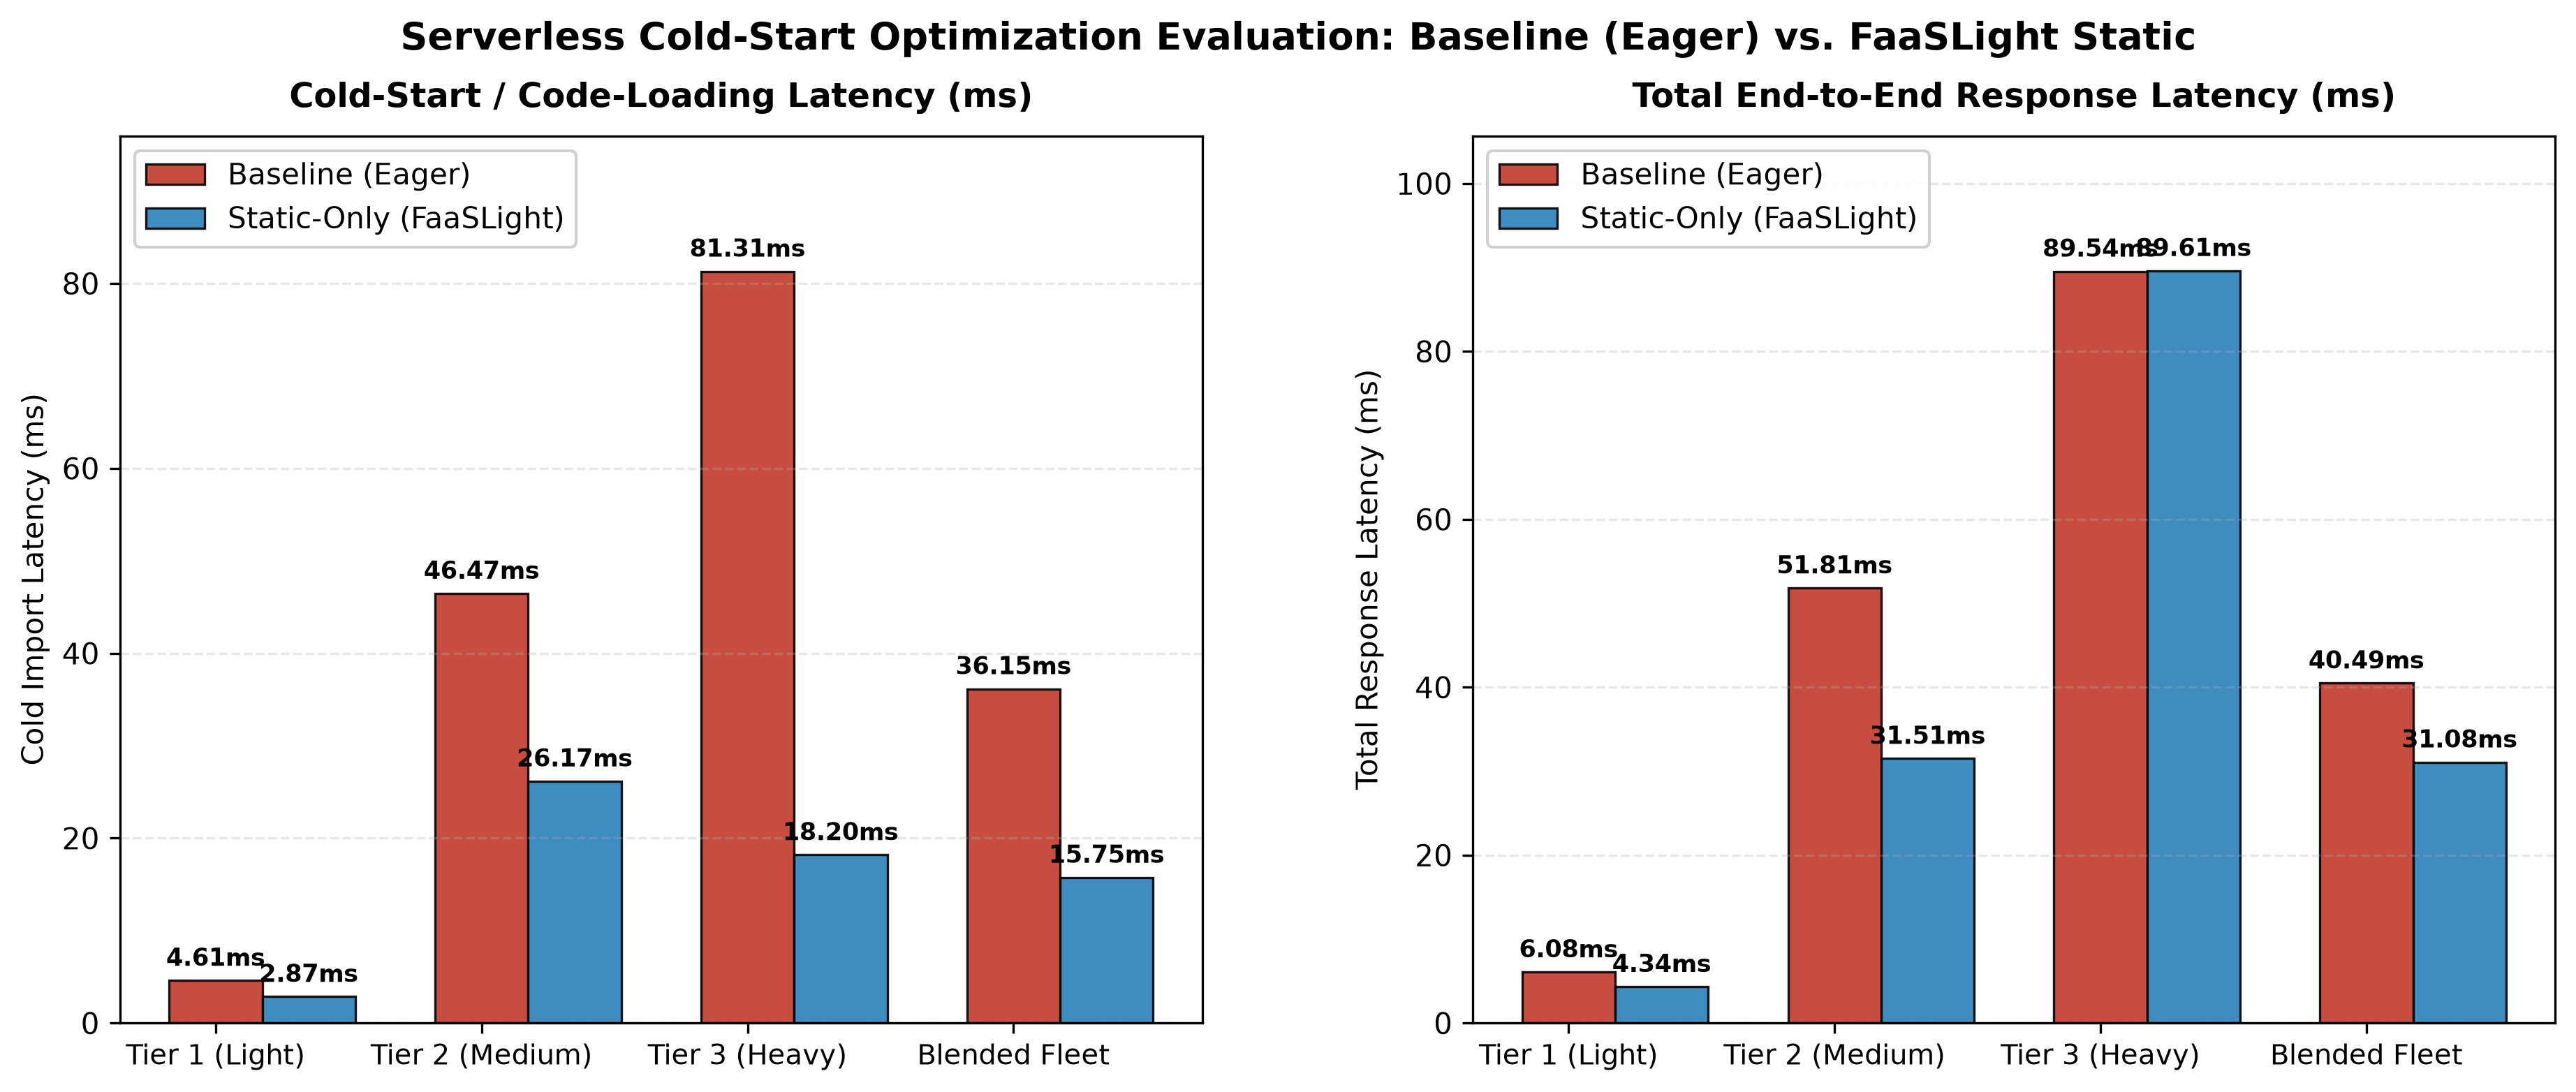
\includegraphics[width=\linewidth]{results/latency_comparison.png}
        \captionof{figure}{Latency comparison across workload tiers.}
        \label{fig:latency}
    \end{minipage}\hfill
    \begin{minipage}[t]{0.48\textwidth}
        \centering
        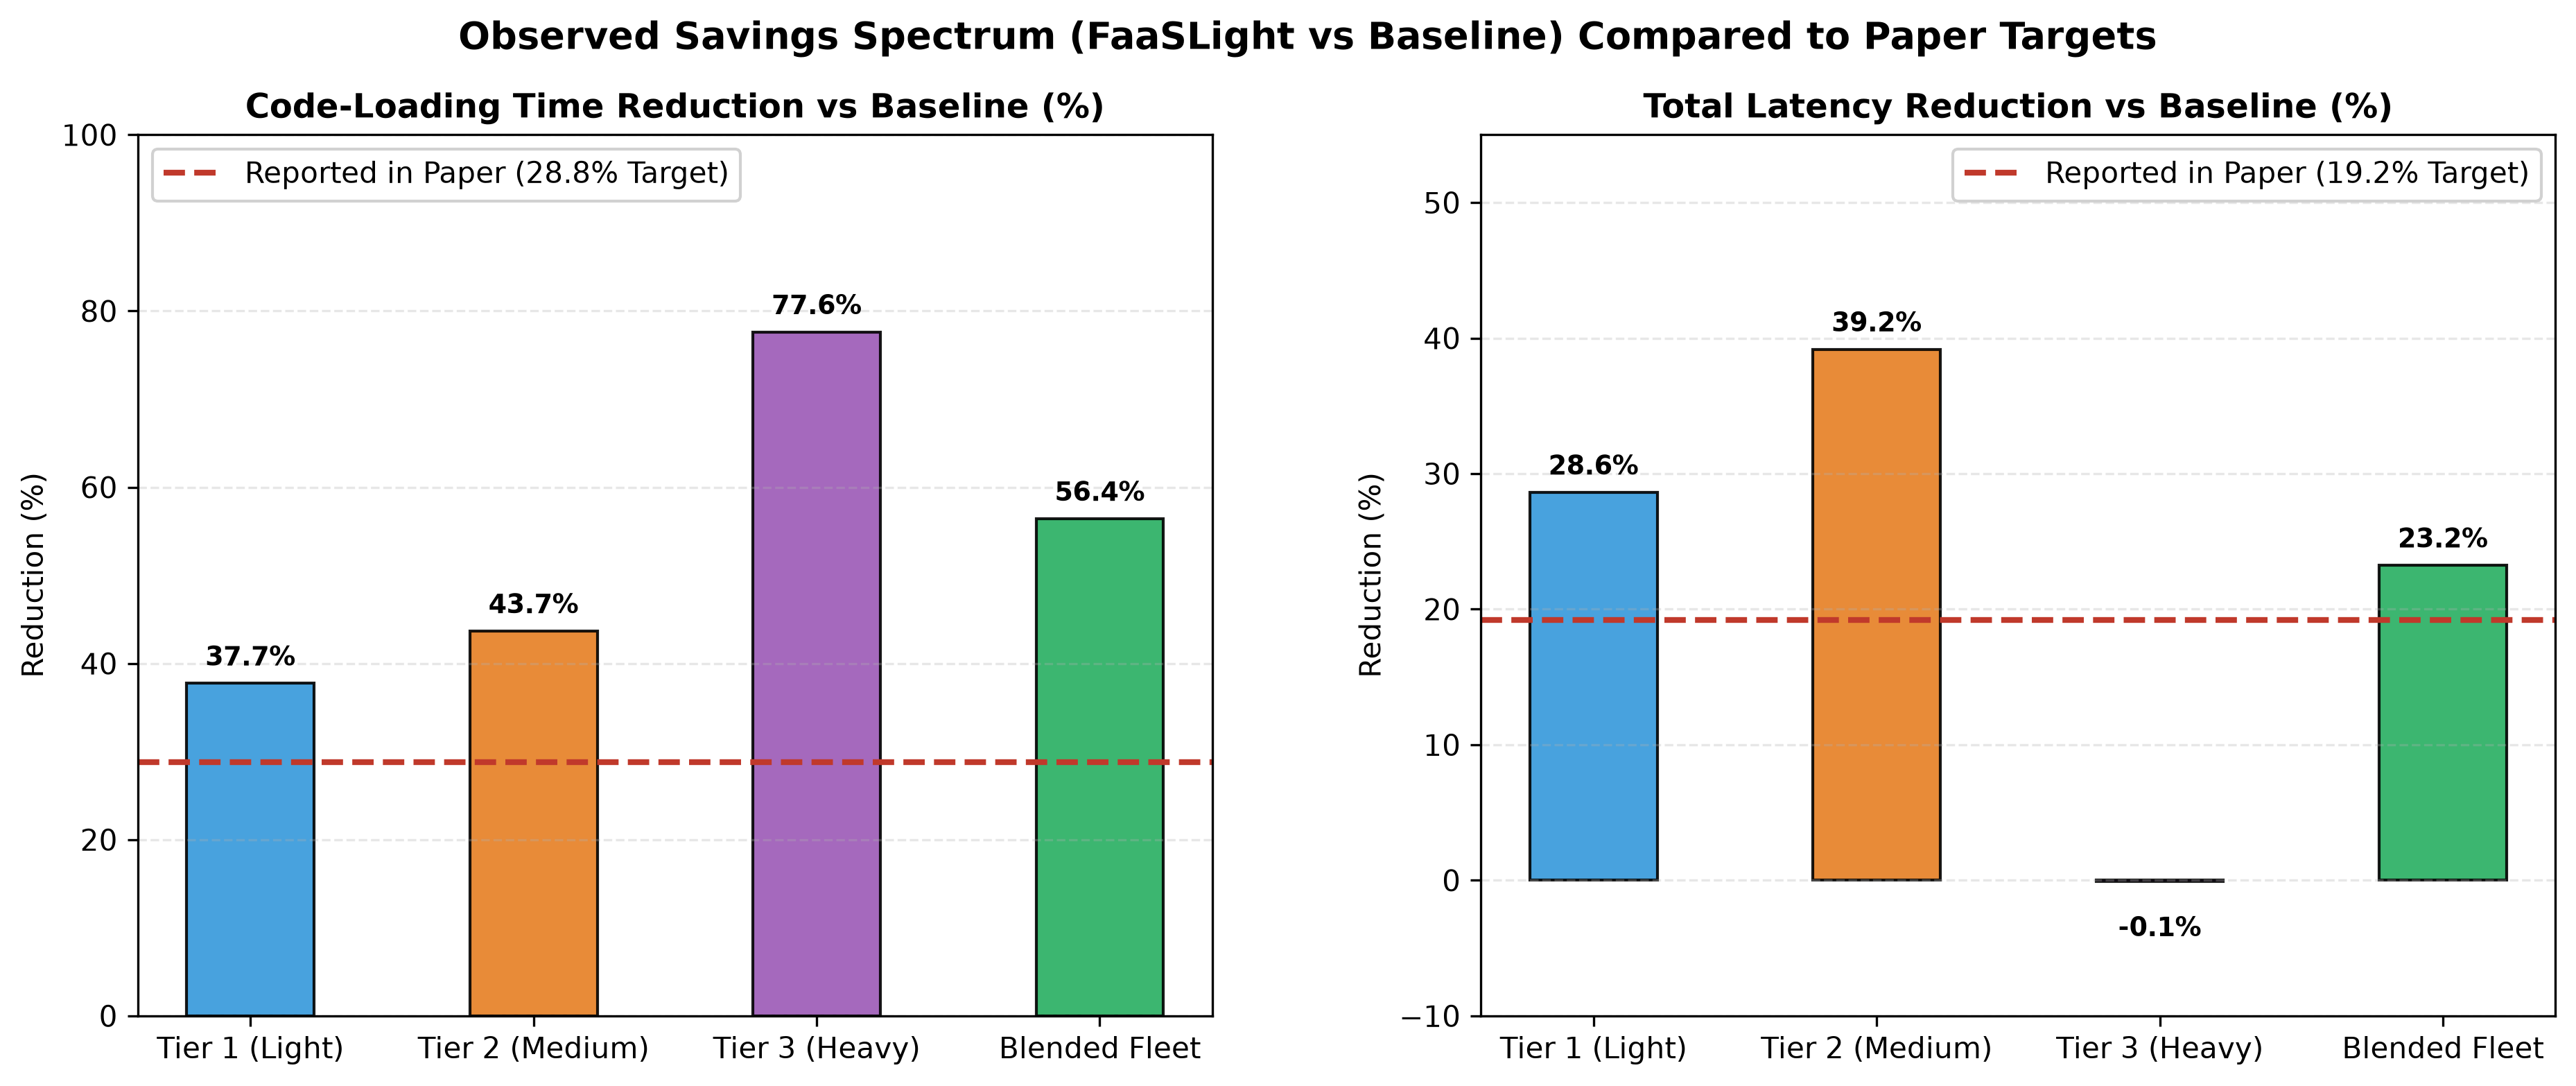
\includegraphics[width=\linewidth]{results/faaslight_vs_baseline_reduction.png}
        \captionof{figure}{Observed percentage reductions.}
        \label{fig:reductions}
    \end{minipage}
\end{figure}

The memory footprint remains nearly unchanged under static deferral. This is expected because the technique changes when a dependency is loaded rather than permanently removing it. The result confirms that the primary benefit is a shorter critical startup path, not a reduction in the total set of application capabilities.

% -------------------------------------------------------------------
\section{Next Work}

The next phase combines runtime transition prediction and dynamic preloading into a single integrated deliverable. The predictor will learn common transitions such as one function routinely being followed by another, and the preloader will use those predictions to warm the next function's optional dependencies while the current request is being served.

The planned work is:

\begin{enumerate}
    \item Connect the predictor to continuous invocation sequences and evaluate it without allowing future observations to leak into earlier predictions.
    \item Integrate prediction with asynchronous background preloading so that preparation stays off the request's critical path.
    \item Compare top-1 and top-$k$ predictions, using confidence thresholds to avoid unnecessary preloading when the sequence is uncertain.
    \item Measure the integrated system using total latency, P95 latency, prediction accuracy, cache-hit rate, and memory overhead.
    \item Add eviction and fallback policies so that an incorrect prediction never affects correctness and does not cause unbounded memory growth.
    \item Repeat the evaluation on shuffled and replayed invocation sequences to study generalization and robustness.
\end{enumerate}

The main success criterion is recovery of the latency currently shifted into heavy request execution, while ensuring that unpredictable workloads do not perform worse than static deferral alone.

% -------------------------------------------------------------------
\section{Conclusion}

This project presents an application-level method for reducing serverless cold-start latency. Static dependency analysis successfully separates essential initialization work from optional request-path work, producing 37.7\%--77.6\% reductions in cold code-loading time and a 23.2\% reduction in average total latency for the blended workload.

The results also establish an important practical limitation. When a heavy optional dependency is needed immediately, static deferral moves its cost from startup into request execution rather than eliminating it. This observation motivates the next phase of the project: predicting likely transitions and preloading the required dependencies before the next request arrives.

The current work therefore provides both a useful optimization and a clear foundation for the predictive extension. The final evaluation will determine whether background preloading can recover the shifted latency with acceptable prediction error and memory cost.

% -------------------------------------------------------------------
\section*{References}
\addcontentsline{toc}{section}{References}
\begin{enumerate}[leftmargin=1.6em]
    \item Y. Liu et al., ``FaaSLight: General Application-Level Cold-Start Latency Optimization for Function-as-a-Service,'' arXiv:2207.08175, 2023.
    \item Amazon Web Services, ``AWS Lambda function lifecycle and cold starts,'' documentation.
\end{enumerate}

\end{document}
